\documentclass[oneside,12pt]{book}
\usepackage[left=2cm,top=1cm,right=3cm,nofoot]{geometry}                % See geometry.pdf to learn the layout options. There are lots.
\geometry{a4paper}                   % ... or a4paper or a5paper or ... 
\usepackage{tabularx}
%\usepackage[latin1]{inputenc}
%fontspec,\usepackage{xltxtra,xunicode}
%\defaultfontfeatures{Mapping=tex-text}
%\usepackage[french]{babel}
\usepackage[utf8]{inputenc}
\usepackage[francais]{babel}
%\usepackage[cyr]{aeguill}
\usepackage{listings}
\usepackage{color}
\usepackage{graphicx}
\usepackage[linktocpage]{hyperref}

\setlength{\parindent}{20pt}

\newcommand\don[6]{
\textbf{#1} \\
(#6) - #2
\begin{itemize}
\item{ \textbf{jet}: #3}
\item{ \textbf{Cout}: #4}
\item{ \textbf{Page}: #5}
\end{itemize}
\vspace{0.5cm}
}

\newcommand\jet[1]{
( Jet: \textbf{#1})}
}
%%%%%%%%%%%%%%%%%%%%%%%%
% Definition des variables
%%%%%%%%%%%%%%%%%%%%%%%%
\newcommand{\Lynn}{\textbf{Etoile Rouge} }
\newcommand{\Jessica}{\textbf{Sagesse Tenace} }
\newcommand{\Luke}{\textbf{Cendre Griffe} }
\newcommand{\Peter}{\textbf{Hurle Mort} }
\newcommand{\Leonard}{\textbf{Sombre Bois} }

%% PNJ
\newcommand{\Monster}{\textbf{Monster Under The Bed} }
\newcommand{\BlackEclipse}{\textbf{Black Eclipse} }
\newcommand{\Tails}{\textbf{Tails} }

\newcommand{\Elisabeth}{\textbf{Elisabeth Lecoeur} }
\newcommand{\Thomas}{\textbf{Zi'ir} }

\newcommand{\Christopher}{\textbf{Christopher} }

%% Meutes
\newcommand{\Night}{\textbf{Night Howlers} }
\newcommand{\Sadness}{\textbf{Sadness Knives} }
\newcommand{\Hidden}{\textbf{Hidden Claws} }

\title{Promenons-nous dans les bois}
\author{Renaud "ObiWan" Guezennec}
\date{}

%\let\origdescription\description
%\renewenvironment{description}{
%  \setlength{\leftmargini}{0em}
%  \origdescription
%  \setlength{\itemindent}{1em}
%}


\begin{document}

\maketitle \clearpage
\tableofcontents \clearpage
\listoffigures \clearpage

\begin{flushleft}
    \chapter{Introduction}
        \section{Lire introduction sur l'univers de loup-garou}
       Les loup-garou sont mi-humain mi-esprit de loup. Il y a très longtemps dans une époque qu'il surnomme la Pangée, Père loup faisait régner l'ordre entre le monde physique et le monde des esprits.\\ Devant son courage, Mère Lune tomba amoureuse de père loup. Elle pris forme humaine pour le séduire. Elle donna naissance à 9 enfants (les premiers nés). De Mère lune ils reçurent la faculté de changer de forme et de Père-Loup la force et l'instinct de chasseur.\\ 
       Au fil des siècles, après la naissance de plusieurs générations de loups-garous, le pouvoir de père-loup perdit de sa vigueur, diluer dans ses enfants et les enfants de ses enfants. Une partie de la meute de Père loup réalisa qu'il était trop faible pour les guider, ils proposèrent leur aide mais Père-loup refusa. Ses enfants assassinèrent Père loup  qui refusait de partager son fardeau avec le fruit de sa chair. Lorsque le coup mortel fut porté, Pere-loup cria si fort qu'il déchira le monde. Depuis lors, le monde des esprits (hisile) est éloigné du monde physique.\\ Les esprits en veulent au loup-garou (uratha) car ils ont cassé leur paradis et on réussi là où ils avaient tous échoué (tuer père loup). Mère-lune maudit ses propres enfants pour leur crime.\\ Depuis, les loups-garous sont sensible à l'argent (le métal le plus précieux au yeux de Mère Lune). Au fil des siècles, elle pardonna, en partie, aux loup-garous qui reprirent le travail de son bien aimé. Le respect de l'équilibre entre le monde des esprits et le monde physique est donc la responsabilité des Loups-garous.  \\
Le monde des esprits est un monde où il fait toujours nuit. Chaque élément du monde physique a son reflet dans l'autre monde à l'exception des humains. Les humains nourrissent par leurs émotions le monde des esprits. Les esprits peuvent être des concept comme la violence, la jalousie l'appétit ou bien des objets esprit d'une porte d'un animal. Les loup-garous sont les seuls êtres autorisé à passer d'un monde à l'autre. \\
\subsection{Les trucs cool d'être loup-garou}
\begin{itemize}
\item Les 5 formes 
\item Locus
\item Régénération
\item Tribu
\end{itemize}

\subsection{Les ennemis}
\begin{itemize}
\item Les esprits : leur but est de grandir le plus possible, 
\item Les purs : Loup garous qui refusèrent de prendre part à la mort de Père-Loup
\item Humains : ils ne sont pas au courant, s'ils apprennent votre existence. Ils vont avoir un projet hostile.
\end{itemize}


\subsection{Serment de la Lune}
\begin{itemize}
\item Les loups doivent chasser
\item Le peuple ne tue pas le peuple
\item Le faible honore le fort, Le fort respecte le faible.
\item Respecte ta proie
\item Le peuple doit vivre parmi les humains
\item Ne mange pas de chair humaine ou de loup
\item Le troupeau ne doit pas savoir
\end{itemize}

  
\section{Les meutes}
\subsection{La Meute PJ: Night howlers}
\Lynn : Lynn Ethwings :  Institutrice (Cahalithe,griffe de sang) \\
\Peter : Peter Torhes : Sherif (Elodothe,seigneur des tempêtes) \\
\Luke : Luke Hereford : Agriculteur (Rahu,maitre du fer)\\
\Leonard : Leonard J. Andrews : Garde chasse (Irraka,chasseur des ténèbres)\\
\Jessica : Jessica  Ethwings: Vétérinaire (Ithaeur,Os de L'ombre)\\

\subsection{La meute sympa mais pas trop : Sadness Knives}
\label{sadnessknives}
\textbf{\BlackEclipse} : Floria Centerfold (alpha, Rahu, chasseur des ténèbres)\\
\textbf{Red Fangs}: David McClurgan  (Irraka, chasseur des tenebres)\\
\textbf{Vicious Pain} : Helen Hallister (Cahalithe, Griffe de sang )\\
\textbf{Fair Wolf} :   Marshall Hereford ( Elodothe, Seigneur des tempetes.)\\
\textbf{Pointed Mind} : Morris Kenneth (Ithaeur, Os de l'ombre )\\

\subsection{La meute bad badass : hidden claws}
\label{hiddenclaws}
\textbf{Winter Mist} : Paul Debian (Alpha, ancien membre de la meute des Sadness Knives, Ithaeur, Os de L'ombre)\\
\textbf{Forest’s Warth} : Clara Haltway(Rahu, Griffes de sang) \\
\textbf{Unwise Wolf} : Casey Jones (Irraka, Griffe de sang,blessé à la main)\\
\textbf{Running Nightmare} : Garry Oakman (Elodoth, Seigneur des tempetes.) \\

\chapter{Les Personnages}
\clearpage
\section{Cahalithe}
\begin{description}
\item[Nom:]{Lynn Ethwings}
\item[Origine:]{Canada}
\item[Auspice:]{Cahalithe}
\item[Tribu:]{Chasseur des ténèbres}
\item[Profession:]{institutrice}
\item[Nom de guerre:]{\Lynn}
\item[Age:]{24 ans}
\item[Histoire:]{ 
Tu es une jeune femme assez timide issue d'une famille riche. Tu as fait tes études d'art et de lettres. Cela t'a permis de voyager un peu partout sur la planète: Europe, USA et Asie. \\
Après tes études, tu t'es installée à New York, pour démarrer une carrière de peintre. Tes peintures se sont vite fait remarquer. Elles décrivaient souvent un lieu sombre avec des formes étranges. Une atmosphère angoissante suintait de ton travail. \\ 
A cette date, ta sœur aînée a pété un câble; Elle a disparu, ne répondait plus à tes appels.\\  Une semaine avant une exposition dans une galerie de la ville, elle est venue te voir.\\
Elle t'a demandé d'arrêter de peindre tes rêves. Tes peintures montraient des choses qui ne pouvait être dévoiler en public. Tu n'as pas compris et l'a envoyé valser. 
La veille de l'ouverture de l'exposition, tu l'as surprise en train de détruire tes toiles. Tu te souviens que cela a réveillé ta fureur. 
Le lendemain, tu étais dans ton appartement et ta frangine avait vidé le frigo. \\
Avec un large sourire, elle t'expliqua que tu étais devenue une loup-garou.\\ Vous êtes parties à la recherche d'autres membres de meute. 
Tu as démontré un certain talent pour localiser des individus proche du \textbf{Premier Changement}. Tu as aidé ta sœur à créer sa meute. Au final, vous avez élu domicile dans un petit village de la campagne canadienne. Tu es devenue institutrice dans ce village pourri.\\
Ces derniers temps tes rêves montrent des pluies torrentielles, des loups massacrés, une chouette qui appelle à l'aide.\\
Le plus étrange, ce sont tes absences. Ce matin (samedi matin), tu t'es réveillée dans ta salle de classe. Tu n'as pas compris ce que tu foutais là. black-out total des événements de la nuit d'hier. Ces moments d'absences sont de plus en plus long et inquiétant. \\
Avis:\\
\underline{\Peter} : Un filou, assez sympathique mais traîne de grosses valises, un jour cela vous pétera à la gueule.\\
\underline{\Luke} : Simple bonhomme il est la force de frappe de la meute. Une personne intéressante mais son manque de culture est parfois lourd.\\
\underline{\Leonard} : son coté solitaire pourrait coûter cher à la meute. Il est efficace dans son métier et dans la meute.\\
\underline{\Jessica}: Ta sœur, elle est la clé de cette meute, son ame. Tu regrettes un peu.\\
}
\item[fiche de perso:]{\href{http://nwod.rolisteam.org/pdf/14}{http://nwod.rolisteam.org/pdf/14}}
\end{description}

\clearpage
\textbf{\large Dons} 
\vspace{0.5cm}

\don{Les bons mots}{+2 en social passif pour encourager ou apaiser}{Aucun}{Aucun}{117}{Réflexe}
\don{Cri de ralliement}{Redonne un point de volonté à ses alliés pendant la bataille}{Manipulation + Expression + Gloire}{1 volonté}{119}{Instantanée}
\don{Canaliser la rage}{Chaque succès permet de sacrifier un tour passé en forme gouru pour obtenir +1 en force ou en dextérité.}{Vigeur + Survie + Pureté}{1 point d'essence}{142}{Reflèxe}

\clearpage
\section{Rahu}
\begin{description}
\item[Nom:]{Luke Hereford}
\item[Origine:]{Canada}
\item[Auspice:]{Rahu/Guerrier}
\item[Tribu:]{Maitre du fer}
\item[Profession:]{Garagiste / Agriculteur}
\item[Nom de guerre:]{\Luke}
\item[Age:]{22 ans}
\item[Histoire:]{
Fils de mère célibataire, tu as souvent vécu avec peu de moyen. Ta mère enchaînait les petits boulots : serveuse, femme de ménage etc.\\
Ton père a abandonné ta mère avant ta naissance.\\
 À l'age de 15 ans, ta mère est tombée malade d'une leucémie. Tu as fait tout ton possible pour la sauver. 
Elle n'avait pas d'assurance et n'a pas pu payer les meilleurs soins. Tu as travaillé très rapidement pour te faire de l'argent pour l'aider, mais cela n'a pas suffi. 
A sa mort, tu t'es enfoncé dans l'alcool et le travail. Un beau jour, tu as reçu un courrier d'un notaire. Il t'a appris que tu étais l'héritier de ton grand-père (père de ton père). Il avait une vieille baraque dans un village canadien, plus un peu d'argent et des terres. Tu y es allé ravi de recevoir un tel cadeau. Ta mère t'a toujours tenu loin de la famille de ton père. \\
Dans le village, tu as ouvert ton garage. Tu répares les engins agricoles ou les voitures. Tes affaires marchent pas trop mal. Lors d'une balade sur tes terres pour sélectionner des arbres, tu as été mordu par un loup. Bizarrement, tu n'as pas ressenti une énorme douleur. \\
La nuit suivante, quatre personnes sont entrées chez toi. Ils t'ont retenu en otage et t'ont parlé de divers éléments pour t'énerver. Visiblement ils connaissaient bien de choses sur toi.  Quand ils ont évoqué ta mère, cela n'a pas loupé, tu t'es énervé. Eux aussi. Tu te souviens vouloir les défoncer. Visiblement, ça c'est pas passé ainsi. \\
Ils se sont excusés mais c'était la seule façon pour eux de te réveiller. Ils t'ont expliqué que tu était un loup-garou.\\
 C'est ainsi que tu as rencontré \Peter , \Lynn , \Leonard et \Jessica . La meute s'est installée dans ton village.
Tu as de bonnes relations avec les habitants, et surtout tu les connais depuis 4 ans maintenant.\\

Avis:\\
\underline{\Peter} : Il est marrant, il semble avoir un passé assez lourd, mais qui n'en a pas ? Puis, c'est un bon partenaire d’entraînement. \\
\underline{\Lynn}: Très sympa, elle te casse un peu les pieds avec sa culture des villes. Elle devrait garder les pieds sur terre.\\
\underline{\Leonard} : Il est de bon conseil, un peu trop concentrer dans son travail (meute ou humain)\\
\underline{\Jessica}: Tu espères sincèrement ne jamais la décevoir. Elle te fait un peu peur. C'est une bonne Alpha.\\
}
\item[fiche de perso:]{\href{http://nwod.rolisteam.org/pdf/90}{http://nwod.rolisteam.org/pdf/90}}
\end{description}
\clearpage
\textbf{\large Dons} 
\vspace{0.5cm}


\don{Redresser}{redresse un objet, réduit les bosses, affecte jusqu'à un metre carrée par tour}{aucun}{1 Point d'Essence}{125}{Instantanée}
\don{Nuit Noire}{coupe les lumières électriques dans une zone (200 mètres carrés par succès), la zone doit être en vue}{Astuce + Larcin + Ruse}{1 volonté}{146}{Instantanée}
\don{Clarté}{+ 5 en initiative}{aucun}{1 Point d'Essence}{137-136}{Réflexe}

\clearpage
\section{Irraka}
\begin{description}
\item[Nom:]{Leonard J. Andrews}
\item[Origine:]{USA}
\item[Auspice:]{Irraka}
\item[Tribu:]{Chasseur des tenebres}
\item[Profession:]{Garde chasse}
\item[Nom de guerre:]{\Leonard}
\item[Age:]{19 ans}

\item[Histoire:]{
Tu es un jeune délinquant. Tu as été traîné de foyers en orphelinats, tu n'as jamais pu tenir en place. 
Tu ne connais pas tes parents.\\ 
Tes petits délits t'ont conduit en centre d'emprisonnement pour jeune (sorte de prison en plus doux). 
Tu as réussi à t'échapper plusieurs fois pour passer quelques nuits à la belle étoile. 
Le cadeau après ce genre de fugue, c'est un bon passage à tabac en règle. \\
Même ces avertissements ne t'empêcheraient pas d'y retourner. \\
Les coups étaient de plus en plus puissant te laissant parfois quelques jours dans le coma. 
C'est là que tu as compris qu'il fallait fuir pour de bon. Tu t'es donc échappé de la prison. 
Tu as été blessé pendant l'opération. Tu as fini dans une grotte que tu avais déjà repéré dans une précédente escapade. Les sensations étaient si pure, tu pouvais entendre le moindre animal respirer, la pluie tombait sur le sol. Ta vitesse t'a beaucoup surpris également. Tu pensais être sauver en arrivant dans cette grotte mais ils t'ont retrouvé.
Tu as entendu s'approcher les gardiens, ils sont rentrés dans ta grotte, tu as hurlé "Cassez vous !". 
Bizarrement, ils l'ont fait. Tu as pu lire de la peur sur leur visage. \\
Le matin suivant, tu t'es réveillé dans l'arrière d'une voiture. À l'avant, deux filles : \Jessica et \Lynn. Elles t'ont pris en charge, nourri et blanchi. 
Elles ont fait annuler les charges contre toi (aux vues des mauvais traitements). Elles t'ont aussi dit que tu étais un un loup-garou. Vous avez fait un bout de chemin ensemble pour trouver les autres. \\
Vous vous êtes installé au Canada. Sur place, tu es devenu garde-chasse, officier des eaux et forêt. Tu surveilles une  partie du parc naturel national. \\ 
Depuis quelques mois, tu fréquentes Elisabeth Lecoeur, une éducatrice venue du Québec.\\ 
Avis:\\
\underline{\Peter} : Un filou, assez sympa mais traîne de grosses valises, un jour cela vous pétera à la gueule.\\
\underline{\Luke} : Simple bonhomme, il est la force de frappe de la meute. Un peu trop cavalier à ton goût, il ne prend pas assez de recul sur les événements.\\
\underline{\Lynn}  : Ses rêves sont une vraie bénédiction pour la meute. Pourtant, elle semble porter le deuil de sa nouvelle nature, tu crains qu'elle soit trop faible pour assurer son devoir envers la meute.\\
\underline{\Jessica}: Tu l'admires, elle dégage un vrai charisme, tu serais prêt à la suivre n'importe où.\\
}
\item[fiche de perso:]{\href{http://nwod.rolisteam.org/pdf/15}{http://nwod.rolisteam.org/pdf/15}}
\end{description}
\clearpage
\textbf{\large Dons} 
\vspace{0.5cm}

\don{Communion avec la forêt}{Transe de communion avec la forêt, le personnage voit 500m à la ronde, et chaque succés ajoute 100m et des informations. Le personnage est inconscient de ce qui se passe dans réellement autour de lui. Il ne peut décrire ce qu'il voit quand le don est actif. Il peut ainsi apprendre la présence d'intru avec un succès, avec trois, il peut apprendre le nombre, le sexe et l'espèce.}{Manipulation + Survie + Ruse}{1 point d'essence}{130-131}{Instantanée}
\don{Pieds de Brume}{Mode passif: -1 pour te pister, Mode actif: -3 (depense d'essence)}{aucun}{1 point d'essence}{114}{Réflexe}
\don{Diriger le feu}{Contrôle un feu, mais ne le crée pas. Le feu peut servir pour attaquer une personne ou tous simplement empêcher le feu de brûler un foret ou augmenter la température pour détruire toute trace. Pour un contrôle fin le test subit un malus de 2}{Force + Survie + Gloire}{1 point d'essence}{109}{Instantanée}

\clearpage
\section{Elodothe}
\begin{description}
\item[Nom:]{Peter Torhes}
\item[Origine:]{Chicago}
\item[Auspice:]{Elodothe/juge}
\item[Tribu:]{Seigneur des tempêtes}
\item[Profession:]{Shérif}
\item[Nom de guerre:]{\Peter}
\item[Age:]{35 ans}
\item[Histoire:]{
Tu étais un avocat d'affaires à Chicago. 
Tu faisais du bon travail et tu as plongé la tête baissée dans le monde de la nuit de cette ville.\\
Tu as gagné quelques affaires qui semblaient perdue d'avance pour des gens du milieu.
Tu as gagné du respect pour cela. Tu as eu accès à de nombreux loisirs: drogue, parties fines, etc. Lors d'une de ces soirées, les deux hôtesses ont commencé à te faire un peu mal. Tu as vu une des deux sortir ses crocs. Ce qui s'est passé par la suite, tu ne t'en souvient pas.  
D'après les informations que tu as eu après coup, l'organisatrice de la soirée a été tué comme une amie à elle. 
C'est après cet événement que tu as rencontré les sœurs \Lynn , \Jessica et \Leonard.\\
Tu venais de subir ton premier changement. Tu es donc devenu loup-garou alors que tu t'amusais avec deux personnes très importante de Chicago.
Elles t'ont accueilli dans leur meute et ont camouflé tes bêtises. \\
En bouquet final, tu as volé beaucoup d'argent a tes clients. 
Tu es parti avec \Lynn, \Jessica et \Leonard pour le Canada. Vous vous êtes installé dans le petit village de Springfield. Ce petit village canadien est un endroit parfait. \\
Tu es devenu le shérif de la ville. Ton boulot est très administratif, mais tu peux faire un peu comme tu veux niveau horaire. 
Au sein de la meute, tu passes pour le vilain petit canard, tu aimerais prouver le contraire. \\

Avis:\\
\underline{\Lynn} : fille coincée, dans son monde, elle te snobe clairement.\\
\underline{\Luke} : Un jeune qui a de la suite dans l'idée, tu es un peu jaloux.\\
\underline{\Leonard} : Il se tuera au travail. Il devrait profiter plus des joies de la vie.\\
\underline{\Jessica} : très surprenante, elle est ton seul vrai soutien dans la meute. \\
}
\item[fiche de perso:]{\href{http://nwod.rolisteam.org/pdf/91}{http://nwod.rolisteam.org/pdf/91}}
\end{description}
\clearpage
\textbf{\large Dons} 
\vspace{0.5cm}

\don{Changement partiel}{permet de changer une partie de son corps dans la forme de son choix: Les bras du gauru ou le museau du loup}{Vigueur + Survie + Instinct primal}{[1 point d'essence]}{121}{Instantanée ou Réflexe}
\don{Voix autoritaire}{Donne un ordre à 1, 2 ou 3 personnes, l'ordre prend la forme d'une phrase complète: «cache ses cadavres dans la ravin près de la rivière», Les cibles obéissent pendant 5 minutes par succès. Un malus de -1 par personne au-delà de la première est appliqué.}{ Manipulation + Intimidation + Honneur vs Résolution + calme}{1 Point d'Essence}{107}{Opposition, résistance réflexe}
\don{Aura de trêves}{Projette une aura de calme, efficace avant que le combat commence. Les personnes doivent dépenser un point de volonté pour commettre un acte violent}{Manipulation + Persuation + Honneur}{1 Point d'Essence}{113}{Instantanée}


\clearpage
\section{Ithaeur}
\begin{description}
\item[Nom:]{Jessica Ethwings}
\item[Origine:]{Canada}
\item[Auspice:]{Ithaeur/Shaman}
\item[Tribu:]{Os de l'ombre}
\item[Profession:]{Vétérinaire}
\item[Nom de guerre:]{\Jessica}
\item[Age:]{26 ans}

\item[Histoire:]{ 
Pendant tes études, tu as subi ton \textbf{premier changement} après avoir surpris ton mec avec un homme. Tu les as tués tous les deux.
La meute locale s'est chargé d'étouffer l'affaire (plus exactement de la faire brûler).\\
Ils t'ont appris ce qu'était les loups-garous. Poussée par une envie de comprendre, tu as enquêté sur ta famille pour y voir quelques irrégularités: des personnes manquantes...\\
Tes voyages ont permis de rencontrer d'autres loups-garous.\\
Tu as compris que la meute d'accueil n'était pas vraiment honnête avec toi. La réalité fut révélée par la suite: c'était des purs.
Après ta période crise d'identité, tu as décidé de reprendre contact avec ta soeur. Il est possible qu'elle ait un rôle à jouer.
En effet, tu l'as retrouvé une semaine avant le début de son exposition dans une galerie New-Yorkaise.\\
Tu lui as demandé de ne pas faire cette exposition. Ces peintures représentaient clairement le monde des esprits.\\
Tu avais peur que tes ennemis l'attaquent. Pour la protéger, tu as détruit ses oeuvres. Tu n'avais jamais vu en colère à ce point.
Elle s'est transformée et vous vous êtes battues. Elle a bien faillit te tuer, ton expérience t'a sauvé. Le lendemain, tu lui as tout expliqué.
Vous êtes parties ensuite à la recherche d'un territoire et de nouveaux frères de meute.\\
Finalement vous êtes arrivés dans le petit village de Springfield au Canada.  \\
Avis:\\
\underline{\Peter} : Il sait lire les gens et n'est pas le dernier dans les combats. Cependant son besoin de richesse et de gloire pourrait un jour lui être dangereux pour la meute. \\
\underline{\Luke} : Petit dernier de la meute. Il te semble encore trop inconscient des dangers qui vous entourent.\\
\underline{\Leonard} : Toujours fidèle au poste. Tu as une bonne amitié avec lui.\\
\underline{\Lynn}: Ta sœur, tu dois la protéger. Elle est trop fragile pour ce monde. Elle t'a bien aidé pour trouver des camarades de meute. Tu sais bien qu'elle prend sa nature comme un fléau.\\
}
\item[fiche de perso:]{\href{http://nwod.rolisteam.org/pdf/35}{http://nwod.rolisteam.org/pdf/35}}
\end{description}
\clearpage
\textbf{\large Dons} 
\vspace{0.5cm}

\don{Langue animale}{Permet de parler avec les animaux pendant une minute avec un animal.}{Manipulation + Animaux + Pureté}{1 point de volonté}{130}{réflexe}
\don{Sentir la malice}{Identifier des sentiments violents: haine, colère.. chez un individu}{Intelligence + Empathie + Sagesse contre Calme et instinct primal}{}{135}{Opposition, résistance reflexe.}
\don{Témoignage de cadavre}{Le cadavre décrit ce qu'il a vu depuis sa mort et les infos ne peuvent pas être plus ancienne que 24h}{Manipulation + Occulte + Pureté}{1 point d'essence}{129}{Instantanée}

\chapter{L'histoire}
\section{Informations à dire aux PJ en début de partie  (ou à rappeler) }

\clearpage

\subsection{Le territoire}
\begin{figure}[!ht]
\caption{\label{territoire} Le territoire}
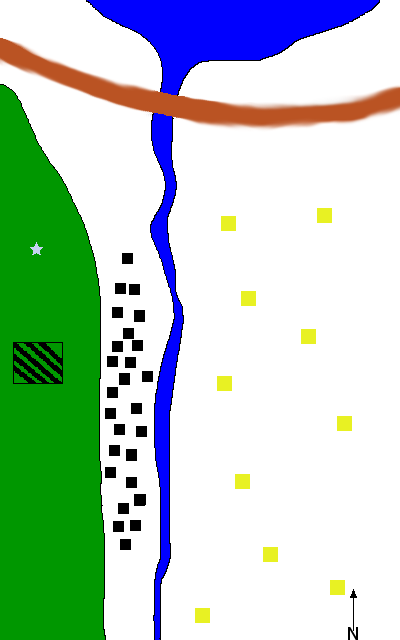
\includegraphics[scale=0.8]{plan.png}
\end{figure}
Il est important de présenter le territoire aux joueurs.
C'est un élément principal du scénario. Il est recommandé de donner une copie de ce plan à vos joueurs (vous pouvez en faire la copie au crayon. En expliquant qu'à l'ouest, il y a le parc national, qu'à l'intérieur il y a une zone interdite. Un esprit très puissant protège cette zone. Au nord-ouest, il y a une mine d'uranium à deux heures de route. Au nord du village, un lac et la grande route. L'est est occupé par des grandes fermes et exploitation agricole. La limite Est du territoire est à 70km du  village, c'est une chaîne de montagne la grande route traverse la chaîne par un col. \\
Au sud du village, le ruisseau prend sa source. Cela monte dans les montagnes. \\

\clearpage

\subsection{Les esprits}
C'est le moment de décrire aux joueurs que les esprits sur leur territoire ne les aiment pas. Cela fait 1 an et des patates qu'ils sont installés et ils n'ont pas de totem. \Jessica n'a pas voulu forcé un esprit à devenir le totem de la meute. Elle attend qu'il y est un candidat. Il y a quelques jours, l'esprit gardien de la foret qui réside dans la zone interdite à envoyer un émissaire à \Jessica. L'esprit Gardien demande à la meute de prouver sa valeur en réalisant le rituel de Chasse Sacrée. \Jessica a accepté le défis. Le rituel a lieu trois jours après la visite de l'émissaire. Ce défi est le premier geste des esprits locaux pour reconnaître la puissance de la meute. 
\begin{itemize}
\item \Lynn : en privée, aborder la questions des absences qui sont assez fréquentes.
\item \Peter : Souhaite devenir maire.
\item \Luke : Rien
\item \Leonard : un Sénateur US et sa famille vont venir lundi pour chasser. Cela demande un petit plus en sécurité. Ils souhaitent faire des chasses bien importante. 
\item \Jessica : C'est le joueur de \Jessica qui doit commencer la partie par un RP. Il doit expliquer à sa meute les événements de la soirée (la chasse sacrée). 
\end{itemize}

\subsection{Les équipements}
\begin{itemize}
\item \Lynn : aucun
\item \Peter : Voiture, et possibilité d'avoir des armes à feu.
\item \Luke : Pick Up, tracteur, et plein d'outil dans son garage.
\item \Leonard : pas d'armes a l'exception un couteau.
\item \Jessica : Moto, klaive, et clinique vétérinaire. 
\end{itemize}

\section{La chasse sacrée}
Le scénario commence un samedi soir.
Les Pj effectuent le rite de la chasse sacrée. Ils chassent un esprit renard/ruse: Tails. \\
L'esprit ressemble à un renard avec les pattes avants bodybuildées. Il a un large sourire, très large un peu à la façon du Chat du Cheshire. La chasse a lieu dans le \textbf{monde des esprits}. Tails part en avance comme le veut le rituel. Il est facile de suivre sa trace (\textbf{Astuce + calme}).\\
\begin{figure}[!h]
\caption{\label{arbre_mort} Refuge de \textbf{Tails}}
\includegraphics[scale=0.8]{scaring_tree.png}
\end{figure}
 En remontant la piste, ils arrivent aux pieds d'un esprit d'arbre mort. Il semble symétrique. Les branches et les racines forment un schéma assez proche.\\ 
L'odeur disparaît dessous les racines. Il est possible de passer sous les racines mais seulement en forme de loup \jet{Vigueur + survie + instinct primal}. Le renard attend dans le creux du tronc, il fera un grand sourire au loup sous lui puis il partira en courant sur une branche et fera un saut géant. Faite une course poursuite selon les règles du monde des ténèbres. Le renard à 23 en vitesse et il jette 7 dés pour la course. Il est normalement très difficile pour les joueurs de le rattraper. Laissez les espérer.\\ 
Après un ou deux tours de course, le renard saute au dessus d'une crevasse. Les loup-garous ne peuvent pas voir ce qu'il y a dans la crevasse, ni sa largeur. Un jet un \textbf{Astuce + athlétisme} permet d'apprendre que le trou fait 3m de large (Trois succès pour le passer). Le but de cet obstacle est de faire perdre du temps. Les joueurs vont probablement réfléchir à deux fois avant de sauter la crevasse. C'est le monde des esprits, il peut y avoir pleins de trucs. En réalité, il n'y a que l'esprit d'un ruisseau. \\ 

Il faut trois succès pour le passer à un test de saut \jet{Force + athlétisme(saut)}.\\ 
Si un personnage tombe, il est mouillé par l'esprit du ruisseau, c'est tout.\\
Quand ils ont fini de passer la crevasse et le ruisseau, et qu'ils se remettent sur la piste du renard, ils ressentent que le rituel est cassé, rompu. S'ils ne sont pas motivés pour retrouver le renard car c'est fini, leur dire que ce n'est pas leur faute, mais que quelque chose s'est passée (s'il ne l'ont pas compris). 

\section{La peur avance}
Ils retrouveront le renard complètement figé par la peur, il tremble et s'est réfugié sous un rocher. Il est très difficile de lui parler (-7). Il est pétrifié. Les joueurs doivent le comprendre. Un jet en \textbf{astuce + survie} permet de remarquer que l’ensemble des esprits environnant est dans le même état que le renard.\\
Le meilleur comprend également que cela dessine une trajectoire vers le village des joueurs. Cela vient de l'ouest. En suivant la trajectoire, il rencontre un esprit (il avance lentement). 

\section{Monstre Sous le lit}
L'esprit ressemble à un tapis de flamme noire. Il y a deux yeux et une bouche dans ses flammes. Il traite les joueurs d'incompétents: « Si je viens ici, c'est que votre territoire me plaît, vous êtes trop nul pour le comprendre ».
Si les personnages essaient de s'approcher, ils doivent réussir à se contrôler:  \jet{Résolution + Calme}, s'ils échouent alors ils passent en rage mortelle, et fuient. 
Le jet doit être fait tous les 2 mètres et le malus augmente à chaque fois. 
A 20m, pas de malus\\
A 18m le malus est de -1\\
A 16m le malus est de -2\\
A 14m le malus est de -3\\
A 12m le malus est de -4\\
etc.\\
Cela ne représente que la capacité passive de l'esprit. Il a, bien sur, des moyens plus actifs de faire peur. Certaines bénédictions présentent un intérêt, l'utilisation pure de son influence. J'utilise personnellement la discipline Cauchemar de \textbf{Vampire: Le Requiem} pour décrire les effets des pouvoirs de l'esprit (Attention, c'est un esprit aucun lien dans le jeu avec des Vampires ).
Seule, \Lynn n'a pas besoin de faire le jet. L'esprit veut lui parler. 
Il l'entoure de flamme noire, et la remercie (en privé) pour son travail, elle gagne un don «Peur mortelle»  qui pétrifie de peur quelqu'un. La personne est libéré à la désactivation du pouvoir ou s'il subit des dégâts (plus d'information voir section \ref{Peur_mortelle}).\\
A ce moment de la partie, les joueurs peuvent avoir compris que c'est un esprit de peur. Cependant, ils ne comprendront pas pourquoi il vient sur leur territoire. Ils chercheront à comprendre et enquêteront dans la forêt, etc. Laissez les faire, ils n'apprendront rien. Rappelez-leur que c'est samedi soir et demain matin, il y a la messe au temple protestant. Le rendez-vous incontournable pour la vétérinaire de la ville, du garagiste, du futur maire et actuel Shérif, du garde chasse et d'une institutrice.\\  
Si les joueurs retournent directement dormir, alors aller au chapitre: La chouette crucifiée (cf. \ref{chouette}). S'ils enquêtent dans la ville, ils découvrent les lésions (chapitre suivant).


\section{Les lésions}
\subsection{Dans le monde physique}
\label{physique_enquete}
Un schéma étrange se dessine dans la ville. La lumière de certaines maisons s'allument (alors qu'il est 2 ou 3 h du matin). Elles restent allumée 20-25 minutes, puis s’éteignent. 
Ceux sont les parents qui vont réconforter les enfants après d'horribles cauchemars.
Si les joueurs décident de parler à une famille, ou à un enfant. Le père de la famille les accueillera avec un fusil (sauf s'il se présente avec leur vrai nom). Nous sommes au Canada, Il est tard et on frappe a leur porte. Dans ce cas, le père dira que son fils ou sa fille a fait de mauvais rêves. Le thème des rêves est très fortement orienté vers les loups (monstres). Les villageois se montreront sur la défensive si les joueurs tentent de rentrer dans une maison en cachette. S'ils tapent à la porte en se présentant officiellement, le ton sera plutôt de la surprise. Ils ne demanderons qu'à aller se coucher et dirons au pj: "A demain matin à la messe".

\subsection{Dans l'hisile}
\label{hisile_enquete}
Dans le monde des esprits, les maisons sont noyées dans une épaisse fumée grise.
Il est possible de rentrer dans une maison dans l'hisile. L'esprit de la maison demandera à se que les loups-garous soignent la lésion pour les laisser passer (ou de l'essence). La fumée vient d'une chambre à l'étage. La fumée descend comme une cascade de l'escalier. Les murs suintent du liquide noir. Le sol est craquelé, comme de la peau brûlée. Il faut essayer de poser une ambiance assez horreur. Les joueurs peuvent suivre la source de la fumée. Cela les guident vers une chambre (d'enfant), bizarrement la chambre n'est pas enfumée. C'est comme l’œil du cyclone. A l'intérieur, il y a 3 esprits : un esprit de sommeil, un esprit de pompier et un esprit d'indien. Ils ont les yeux complement rouge et la peau déformée. Ils attaquent à vue la meute. Le combat est assez facile cependant les joueurs ne seront pas plus avancés. S'ils font plusieurs maisons, ils découvriront la même chose (changé un peu la description des esprits dans chaque maison, mais tous ont muté et sont agressif). Les détruire n'arrange rien.  (Caractéristiques des esprits voir \ref{esprit_mutant}). 

\section{La chouette crucifiée}
\label{chouette}
En rentrant chez lui, \Peter découvre qu'une chouette est crucifiée sur la porte de la maison. Elle a été cloué à sa porte vivante et est morte en se vidant de son sang. C'est une espèce protégée \Jessica ou \Leonard pourra lui donner l'information. Laisser le gérer la chose, il peut appeler les membres de sa meute ou gérer cela tout seul.

\section{La messe}
Le dimanche matin, la ville entière se donne rendez-vous au temple pour la messe et se montrer (Détailler un peu la relation religion/loup-garou). 
Le maire accueille l'ensemble des personnes avec son neveu Julian. Il présente son neveu au village. Il vient effectué un stage. Le maire est clairement en campagne électorale, avec 3 mois d'avances. Ils invitent tout le monde à un pique-nique après la messe.
Le serment du pasteur évoque dieu comme un berger, qui protège ses moutons contre les loups. Si vous vous y connaissez, faites-vous plaisir. \\ 
Des trucs clochent, les personnages peuvent remarquer quelques points: \\
Le maire de la ville est très bien habillé (d'habitude, c'est plutôt un bouseux en salopette).\\ 
L'ambiance n'est pas trop à la joie (\textbf{jet caché d'empathie + astuce})\\  1 succès = Truc louche,\\  2 succès = les gens sont fatigués et stressés,\\  3 succès = les enfants sont absent, cela manque de bruit.\\
Musique: Gospel ou l'hymne du Canada.

\section{Pique-nique après la messe}
Après la messe, le pique-nique commence, le maire fait discours. Les assistants de \Peter glisse un petit mot au maire et à \Peter. Le jeune assistant de \Leonard lui transmet également un fax. C'est un avis de tempête sur la ville. Elle commencera ce soir vers 20h et durera jusqu’à 2h du matin. Le maire prend un mégaphone pour communiquer l'information. Tout le monde part pour aller barricader sa maison. 
Les joueurs doivent faire pareil. La copine de \Leonard, \Elisabeth lui demandera de l'aide. \Luke sera aussi pas mal sollicité. Faite leur gérer cela: \textbf{Astuce + Artisanat}.  \\

Vous pouvez placer quelques événements mineurs: Des villageois informent les joueurs qu'il y a des traces de loup un peu au sud du village (vers la montagne). C'est trop tôt dans la saison pour les voir si bas des montagnes.
Puis vient le gros événement, les \textbf{Hidden Claws}.

\section{Le hurlement des Hidden claws}
Le dimanche vers 17h, Les PJ entendent des hurlements qui les appellent.  Le hurlement dit "Les \Hidden souhaitent rencontrer les \Night, attendons à la frontière du territoire".
Il est émit à l'est (à environ 70km, la frontière de leur territoire). Il est préférable d'y aller en véhicule par la grande route. 

\section{La rencontre avec Hidden claws}
Le lieu de rencontre est un petit col en haut d'une colline, à la frontière Est du territoire. C'est la seule route pour passer cette chaîne de collines.
Les PJ rencontrent la meute des \Hidden.\\ Ils sont 4, 3 hommes et une femme.
Les \Hidden expliquent qu'un membre de leur meute est devenu fou. Il a tué de nombreux humains, et a violé beaucoup de points du serment de la Lune. Il est devenu un \Thomas. Un loup garou ayant une harmonie de 1 ou 0. \\
Les \Hidden pensent que ce danger est sur le territoire des joueurs. Ils préfèrent prévenir. Les \Hidden resteront polis, pour ne pas attirer l'attention des joueurs. \\
Un des membres de la meute est blessé, il lui manque deux doigts (annulaire et auriculaire de la main gauche). Il se justifie en disant que c'est le \Thomas qui a fait cela, il lui a mangé les doigts. Les \Hidden donneront une photo en forme humaine du \Thomas.\\
Si les joueurs invitent les \Hidden, ils refuseront poliment. Si les joueurs insistent, ils accepteront mais partiront dès que possible.
Quand les joueurs retournent au village, la tempête fait déjà rage. Vous pouvez tester leur conduite \jet{Dextérité + Conduite} avec un malus pour le mauvais temps. J'utilise aucun malus s'ils ont pris une voiture. Si \Jessica a pris sa moto, j'applique un malus de -2 dés.\\
Bref, les joueurs rentrent au village alors que la tempête arrive vite. Le village est comme mort. A ce moment là, normalement vous avez croqué le cerveau de vos joueurs.  
Musique: Tension


\section{Pendant la tempête}
Vous pouvez ici jouer quelques scènes d'actions, facultative.\\
Soit:\\ 
\begin{itemize}
\item  \Elisabeth joue à des jeux sado-maso avec \Leonard (elle pourrait voir sa régénération surnaturelle, attention à la lubie).
\item \Elisabeth est possédé par l'esprit de peur (\Monster) et elle obtient une voie qui pétrifie \Leonard. Il ne revient pas vers les autres à la fin de la tempête. Les autres joueurs s'inquiéteront de son absence.
\item \Peter apprend qu'un enfant a fuit sa maison pendant la tempête. La meute ira certainement le sauver.
\item Un incendie se déclare à la fin de la tempête, il brûle une maison et menace de se répandre à la seule pompe à essence du la ville. 
\end{itemize}
Quoi que les personnages font, ils peuvent faire un jet d'\textbf{Astuce + Calme}. Ils entendront une meute de loups assez importante hurler. Les hurlements s'arrêteront assez brutalement. La tempête continuera quelques heures après les hurlements. \\
Si les personnages sortent pour enquêter dans la tempête, faites les souffrir. C'est une très mauvaise idée de sortir pendant une tempête. S'ils y vont pour sauver un enfant vous pouvez être plus sympa. L'enfant ne se sera pas enfoncé trop loin dans le parc naturel.\\
C'est à vous de meubler ce passage ou de le faire vite passer.

\section{Une meute de loup est retrouvée morte}
\label{MeuteMorte}
Les personnages voudront probablement enquêter sur cette meute, après la tempête. C'est peut-être elle qui vient proche du village et fait peur à des enfants? (ce n'est pas sur que les joueurs aient compris cela) \\
Il est difficile de s'orienter dans la foret après la tempête \jet{Astuce + Survie}. Au termes de leur traque, ils trouveront des cadavres de plusieurs loups dans la forêt du parc naturel. \\
Enquêter leur permet de comprendre les choses suivantes \jet{Astuce + Survie ou investigation} : \\
-Une louve de la meute est encore en vie.\\
-Dans un recoin, un loup blessé s'était réfugié (une odeur de sang mais la tempête a effacé toutes les traces).\\ 
-La meute l'a encerclé pour attendre sa mort avant de le manger.\\
-Les loups ont perdu patience et il y a eu un combat. Le loup(-garou) a pris une forme plus forte (gauru). 
il est passé à l'attaque. Il a détruit la meute de loup. Certains loups de la meute se sont enfuit. \\
La rage mortelle de l'individu peut troubler les esprits environnant. Ils ne seront pas coopératif et critiqueront l'efficacité des joueurs. Si un don quelconque est utilisé pour revoir la scène, l'image devient noire. L'esprit a eut peur, il a "fermé les yeux".\\
L'utilisation de langue animale et témoignage de cadavre permet d'avoir la fuite du \Thomas.\\
-Il y a un schéma qui se dessine dans la foret. Le loup-garou ne semble pas avoir tué volontairement les loups. Beaucoup sont morts écrasés sous le poids du gouru. Après s’être transformé, il a pris la fuite vers l'ouest (extérieur de territoire des joueurs). \\
1 - Il a perdu sa forme gouru après 50 mètres.\\
2 - Il se cogne contre quelques arbres et avance difficilement en zigzagant.\\
3 - Il se transforme en gouru. Il plie des arbres sur son passage en gouru. (on repart sur l'étape 1).\\
Ce schéma est répété plusieurs fois, puis la trace remonte dans la montagne, il y a plus d'arbre et que des rochers, la pluie a tout effacé. De plus, la trace se perd à quelques centaines de mètres de la fin de leur territoire.\\

A ce moment, il y a deux possibilités. Soit vos joueurs voudront continuer sur la piste même si elle est perdue (la direction générale mène vers la frontière du territoire). Soit ils voudront sauver la louve.\\
Dans le premier cas, vous pouvez aller directement consulter le chapitre: \ref{sadness}, sinon aller voir \ref{louve}.
Musique : Foret 



\section{La louve}
\label{louve}
Un jet de \textbf{dextérité + médecine} pour soigner la louve est possible. 
La louve a perdu une patte, ce détail est important. \\ 
Cette étape est juste, un moyen de décompresser un peu et de regrouper la meute, si elle ne l'était pas. C'est très probablement la vétérinaire qui voudra soigner la louve. Une meute part rarement en chasse sans son alpha. Le temps de gérer la louve. C'est le lundi matin. Il faut gérer les conséquences de la tempête [chapitre: \ref{consequence} ]. \\


\section{Tempête: les conséquences}
\label{consequence}
Cette section est un peu un moment bac à sable. Si vos joueurs ont raté des indices, c'est le moment de la séance de rattrapage. \\
-Vous pouvez jouer le chapitre \ref{hisile_enquete}. S'ils n'ont pas visité de lésions avant.\\
-Pareil pour \ref{physique_enquete}, les gens se montrerons sûrement plus bavards. Il est possible d'apprendre que certains enfants parlent d'un loup à leur fenêtre. Une enquête [ jet : \textbf{Astuce + investigation} ] montrera qu'un loup-garou en Urshul s'est agrippé au rebord de la fenêtre. Il regardait dans la chambre.\\
-Certaines familles vivants dans le sud [dans les montagnes] parleront de loup à 3 pattes qui pillent les poubelles.\\
-Les plus gros dégâts sont enregistrés chez la famille: Porkman. Ils ont des triplés. Les enfants jouaient dans la grange, quand elle s'est effondrait, 
ils ont eut le temps de partir dans la maison (en bois), qui s'est effondré à son tour. Ils se sont réfugiés dans la dépendance en brique de la maison.\\
Il ne faut pas hésiter à demander aux joueurs d'avoir des idées pour calmer les peurs des enfants. La tempête a ravagé la ville. Les lésions sont encore plus grandes. Atelier peinture, réunion d'informations, tout est possible mais rien ne marchera vraiment mais c'est mieux que rien.

\section{Le sénateur du Texas chasse}
Le lundi à midi, le gouverneur arrive avec sa fille et son futur gendre. Ils vont chasser en forêt. \Leonard doit les accompagner vers un point de vue où ils s'installeront pour chasser. Le père et la fille savent chasser et ont l'habitude des armes. Le gendre est beaucoup moins à l'aise. 
La forêt est en bordel, \Leonard doit réussir un jet de \jet{Astuce + Survie} pour trouver une route vers la zone. \\
Le sénateur va voir une chose au loin et va tirer. \\
Sur le chemin, le gendre identifie des traces bizarres. C'est gris. On en voit sur des trons et par terre. Le gouverneur (un homme rond et vieux) pense que c'est des excréments d'animaux mais ne connaît pas le type. Si \Leonard (ou un autre loup garou) touche cette subtance, cela chauffe dans ses mains. S'il le renifle, il se prends un dégât aggravé et un mal de tête monstrueux. Il ne faut pas oublier de faire un jet de rage mortelle. La transformation en gouru annule les malus de douleur et détruit l'argent de l'organisme.\\
\Leonard porte le gros du matériel. Ils laissent les 3 chasseurs dans un point de vue et repart.\\
Cette scène est un moyen de raccrocher les joueurs sur la piste du Monstre (le Zi'ir). Si vous voulez la rendre plus intense, vous pouvez. Vous pouvez soumettre l'idée que \Leonard demande à la meute de se réunir vers la piste pendant que lui, finit avec les chasseurs. 


\section{Sur les traces du \Thomas}
Le beau temps et les blessures du \Thomas le trahissent. Il est maintenant possible de le suivre et de comprendre un peu son comportement. En fait, il vient dans la forêt pour se nourrir mais ne vit pas sur le territoire de la meute mais juste à la frontière. La trace identifié par Léonard mène droit vers la grotte. Les joueurs seront très enthousiaste à l'idée de l'attaquer.
Ils vont vite déchanter (voir \ref{black_eclipse} ). 
Quand vos joueurs auront retrouver les traces qui mènent vers le \Thomas, laisser leur le temps de se regrouper pour élaborer une stratégie. Le \Thomas est dangereux dans leur tête (c'est le boss de fin pour eux). 



\section{\BlackEclipse attaque}
\label{black_eclipse}
Les personnages courent en suivant la piste du \Thomas. Elle mène vers l'Ouest du territoire. Quand ils ne sont qu'à quelques kilomètres de la fin de leur territoire, faite leur faire \textbf{un jet d'Astuce + Calme - malus d'environnement} (Si un personnage est en avant par rapport aux autres, C'est lui qui fait le jet et subit l'attaque). Ce jet permet de savoir s'il est surpris (pas de défense) ou non. Heureusement pour eux, il n'y a qu'un attaquant. \\
\BlackEclipse aura le temps de faire une seule attaque (Elle a l'initiative obligatoirement, au premier tour). Elle est en forme gauru et elle attaque avec ses griffes, elle n'a que 12 dés d'attaques. Elle ne tuera pas volontairement, son but est de les interdire de remonter la piste. Elle veut protéger son fils (le Zi'ir).\\
Quand elle a attaqué, elle est assailli par deux loups-garous en forme \textit{Urshul} (\textbf{Vicious Pain et Red fangs} (voir \ref{sadnessknives})), les deux autres se positionnent en Dalu entre le trio et la meute des joueurs. \textbf{Fair Wolf} utilisera \textbf{Aura de trève} pour calmer tout le monde.
\BlackEclipse va se calmer et se changer en Dalu. C'est une femme d'environ 40 ans, très musclée. Elle a vraiment une tête de vétéran. Dans son dos, une hache immense, un fétiche très très puissant (voir \ref{devoreuse} ). Elle ne parle pas avec la meute des joueurs et s'éloigne un peu. Elle passe ses nerfs sur un arbre. Elle gronde vers \textbf{Fair Wolf} en disant "qu'ils n'ont pas à intervenir dans cette histoire". \\ 
\textbf{Fair Wolf} se présente comme le porte parole de la meute des \textbf{Sadness Knives}. Il demande à tous de prendre une \textbf{"forme plus propice au dialogue"}. Quand les joueurs sont en forme humaine ou dalu, faite faire un jet en \textbf{Astuce + Empathie} à tout le monde sauf \textbf{Cendre Griffe}, un succès indique qu'il y a un air de ressemblance entre \textbf{Fair Wolf} et \textbf{Cendre Griffe} (Attention, le joueur de Cendre Griffe, ne doit pas savoir le résultat du test). \textbf{Fair Wolf} va prendre quelques secondes en regarde \textbf{Cendre Griffe} pour lui dire :  {\Large \textbf{Luke, je suis ton père}} avec une petite musique dramatique en fond. \\
Passé cette référence, \textbf{Fair Wolf} demande pardon pour avoir franchi le territoire des joueurs et il lâche des infos. \\
Il explique qu'il y a 10 ans environ, ce territoire était celui de sa meute.\\
Un jour, ils sont partis à la chasse à l'extrémité du territoire, à leur retour, l'enfant de \BlackEclipse avait disparu. Elle est devenue folle et a détruit définitivement le totem de la meute, un esprit Ours/force avec sa hâche. \\
Le totem avait pour mission de protéger l'enfant. Cela a traumatisé les esprits de la zone. Ils ont abandonné le territoire et sont allés s'installer dans Ouest (a des milliers de kilomètres). Il y a quelques jours, \BlackEclipse a eut des visions et elle est retombée dans sa folie à propos de son fils. Ces visions lui montraient son fils adulte dans le village des Joueurs. Elle a donc quitté le territoire pour se rendre ici. Il est important d'expliquer qu'elle est dans la zone depuis plusieurs jours. Elle a été rattrapé par sa meute, qui lui a fait entendre raison. Elle repartait quand elle a entendu le coup de feu (tiré par le sénateur). 
Elle a voulu aller voir et a trouvé les \Night. \\
C'est une petite astuce pour expliquer pourquoi, elle apparaît maintenant et pas avant.\\

\section{Black Eclipse Vers son fils}
Laissez vos joueurs réfléchir avec les nouvelles données qu'ils viennent d'obtenir. 
Si cela traîne trop, les \Sadness demanderont au joueurs de les accompagner à la frontière pour leur montrer qu'ils ne sont pas des ennemis. Les deux meutes suivent donc la piste, \BlackEclipse pense que c'est son fils, mais rien n'est sur.\\ 
Si les joueurs parlent, des \Hidden et montre la photo. \BlackEclipse prendra la photo et tombera en larmes. \\
A la frontière du territoire,  les deux meutes se séparent.\\
Il est temps de recentrer l'action sur l'esprit de peur. Il y a plusieurs possibilités soit vous relancez un peu l'enquête sur l'esprit de peur soit vous déclenchez le chapitre suivant. \\
Personnellement, je profite de ce temps pour faire un point avec les joueurs de ce qu'ils savent et des interrogations qu'ils ont. \\


Après que les joueurs ont réfléchi à un plan d'actions et qu'il redescende vers le village. Lancez la suite!


\section{Fin possible}
Cette section a pour but de vous donner un peu de recul face à l'histoire. A ce moment de la partie, vous joueurs auront compris (à tord) que \Thomas fait peur aux enfants du village. Il n'est pas la seule cause des peurs et c'est à vous de le faire comprendre aux joueurs, ou du moins d'essayer. Ne les laissez jamais rester trop enquêter sur la même piste. Ils vaut mieux les mélanger un peu. La fin que je propose est une fin possible qui me semble raisonnable. Sentez vous libre de la modifier. Je fais le choix délibérer de ne pas faire un grand combat épique à 3 meutes (ou 2) cela serait bien trop long. Je laisse un adversaire dangereux, voir: \ref{ausecours}.
Vous pouvez faire le choix de laisser 2 adversaires au lieu d'un. J'aime que \textbf{Winter Mist} s'échappe cela sert de Cliffhanger au scénario. Partez du principe que l'action des joueurs peut changer la donne. C'est difficile mais rien n'est impossible.

\section{Night Howler au secours!!}
\label{ausecours}
Cette scène est à placer au bon moment dans la partie. Elle peut intervenir le lundi matin juste  après la scène \ref{black_eclipse} ou bien après. 
Ils apprennent que des quelques choses ne va pas. Cela peut être \Tails l'esprit de la foret qui les prévient que des loups-garous sont passés par leur locus. Cela peut être des coups de feu tiré par le sénateur alors que les joueurs sont dans la forêt. Cela peut être un hurlement de demande à l'aide. \\
Des loups-garous ont utilisé leur locus pour passer de l'hisile au monde réel et ont pris direction plein Ouest. Ils sont 4. Que les joueurs remonte la piste ou courent pour aller aider les personnes qui les appellent à l'aide. \\
Ils vont aller au delà de leur territoire. En redescendant la chaîne de montagne, ils vont voir de loin une scène d'horreur. 
\textbf{Winter Mist} est derrière \BlackEclipse. Elle est à genoux et sévèrement blessé. Les personnages courent dans la direction de la zone mais ils sont encore trop loin. Ils voient \textbf{Winter Mist} décapiter la pauvre femme et mordre dans la joue de la tête découpée. Il a visiblement orchestré la scène pour que les joueurs voient ça. Il parle à un membre de sa meute (Unwise Wolf) qui se met en position et attend les personnages toutes mâchoires et griffes en argent dehors. \textbf{Winter Mist} et un autre membre de sa meute utilisent la vitesse de père loup pour s'enfuir. Il faut gérer le combat et/ou la course poursuite.  

\section{La scène de crime}
Une fois le combat terminé, les joueurs vont probablement avoir envie de comprendre ce qui s'est réellement passer. Il y a un membre des \Hidden mort par terre. Quatre membres des \Sadness sont morts. Il manque donc une personne \textbf{Vicious Pain}. 
Laissez les gérer la scène de crime \jet{Astuce + investigation (scène de crime) }. Il est possible de comprendre que les \Hidden sont tombés par surprise sur les \Sadness. Ils ont utilisé des armes en argent visiblement. Ils étaient clairement bien préparer. La hache est brisée et l'esprit a été libéré. \textbf{Vicious Pain} n'est pas là. Son corps est un peu plus loin devant une grotte (\ref{chirurgie}). potentiellement dire qu'il est toujours bon d`enterrer des Uratha et leur rendre un dernier hommage. S'ils n'ont pas réalisé qu'il manque une personne ou s'ils ont fait pas mal de succès pour enquêter. 

\section{Chirurgie au Klaive}
\label{chirgurgie}
Le \Thomas est dans une grotte, il est difficile d'y voir un truc sans s`approcher. Il a un comportement assez étrange. Il change de forme assez continuellement: de forme humaine, urshul, dalu et Gauru. Une énorme bosse est visible dans son dos. Il se jette contre la paroi de la grotte, la bosse en avant. Il est évident que cela provoque de la douleur.   Un jet en \textbf{Astuce + Occultisme} permet d'identifier les marques d'un rituel dans les tatouages entourant la bosse.
Normalement, ces informations devrait suffire aux joueurs pour comprendre qu'ils peuvent sauver le \Thomas. Il faut qu'il l`immobilise. C'est à \Jessica de faire le travail probablement.
Ce n'est pas compliquer. Ils peuvent prendre quelques dégâts dans l'opération mais rien de méchant. 
  


\section{Les enfants}
Le lundi matin ou le mardi matin.
A ce stade, les joueurs auront compris que c'est la peur des enfants qui nourrit l'esprit.
Dans le monde des esprits, l'esprit est beaucoup plus gros, il se multiplie formant comme un réseau pour absorber l'ensemble de l'essence. Il entretient la peur. En général, les joueurs commencent à fatiguer et veulent du réel. Il est important de finir une ou deux intrigues. Laissez les joueurs avoir de l' imagination, pour faire parler les enfants. Il est possible d'apprendre que certains enfants rêvent de la même chose. 
Un loup a 3 pattes, un loup à leur fenêtre, des loups dans la forêt s'approchant des maisons. Il est possible qu'un des rares élèves présent le lundi ou le mardi signale le tableau bizarre dans la classe de \Lynn . 

\section{Le tableau dans la classe}
Pendant l'absence de \Lynn le vendredi soir. Un esprit lui a fait placer un de ses tableaux dans sa salle de classe. \Lynn est incapable de le voir. Les enfants ne le verront qu'à partir de Lundi. Tous les enfants présents le lundi ne seront pas là le jouer suivant. 
Il est possible que le joueur de \Lynn décide de parler des ses moments d'absence aux autres. 
Si \Jessica apprend pour le tableau, vous pouvez lui faire faire un \textbf{jet de rage mortelle} contre \Lynn . Si les joueurs parlent avec des enfants qui auraient vu le tableau, ils auront grandement peur de \Lynn .
Si le joueur de \Lynn ne parle pas, consultez la section \ref{directeur}.

\section{Directeur de l'école}
Cette scène peut être joué à partir du mardi matin. C'est une section bonus pour donner des indices. Il est très rare que la démarche des joueurs auprès des enfants leur permette d'apprendre cela. 
Le directeur aura reçu beaucoup de courriers ou de coups de fil. Des parents d'élèves ont rapporté que le nouveau tableau dans la classe leur faisait peur. Le directeur confirmera que le tableau n'a rien à faire dans une salle de classe et demandera donc des explications à \Lynn. Il est possible pendant l'interview avec le directeur de voir que \Elisabeth est aussi concerné par les demandes des parents d’élèves.


\section{le cas \Elisabeth}
Son emploi du temps avec les enfants est simple. Elle leur lit des contes en français tous les après midi. Elle est influencée par \Monster . Il lui donne un pouvoir de manipulation des rêves. Si elle dit quelques choses, la personne rêves de ce que \Elisabeth dit. Les contes qu'elle lit sont assez sanglant et triste. Les élèves ne comprennent pas tout mais le pouvoir n'a pas besoin de ça. \\ 
Elle est très attaché à un livre. \\ 
\Monster fait en sorte qu'\Elisabeth aime particulièrement ce livre de conte (une copie d'un ouvrage du 14ème siècle). Il est en français donc il faut faire un jet en \textbf{Intelligence + Erudition}. Seul \Peter et \Lynn ont des notions de français. \\

Du coup, si \Elisabeth parle à \Leonard de jeu sexuel qu'elle voudrait expérimenter, il rêvera de cela. \\

Il y a plusieurs moyens de gérer son cas. Les PJ peuvent décider de la tuer. Il peuvent juste l'enfermer loin des enfants que son influence diminue. \\ 

\section{Les Loups dans la ville}
Des meutes de loups semble de plus en plus s'approcher des habitations. Ce chapitre peut être jouer le dimanche après midi ou pendant la tempête avant la section \ref{MeuteMorte} .
Un père de famille a été tué par une meute alors qu'il était sortie pour une raison quelconque. 
La meute est rentré, à tuer toute la famille ou presque. Un enfant a survécu. Il témoignera qu'un Grand loup a combattu les autres et les a repoussé.\\
Cette scène n'a jamais été joué mais je pense que c'est une bonne idée. Pour des raisons de cohérence. j'imagine assez bien que la meute responsable de ça, soit la même que dans la scene \ref{MeuteMorte} . Ce n'est pas obligatoire mais il faut laisser des indices pour inculper ou disculper la louve: Présence d'un loup à 3 pattes. \\ 
Je pense que la scène doit avoir lieu avant la scène \ref{MeuteMorte} mais les PJ pourrait l'apprendre après.  \\
C'est évidemment \BlackEclipse qui aura sauver le petit enfant de 8 ans de la maison. La meute aura fuit devant la présence du loup-garou. L'enfant sera terrorisé, difficile d'en apprendre de lui mais des cadavres de la maison, c'est une autre paire de manche. 

\section{Les sadness knives}
\label{sadness}
Pour jouer cet événement, les joueurs doivent être tous ensemble.\\
Il est important de jouer cette scène avant qu'il rencontre le Zi'ir.\\ 
Le jeu est de montrer les tensions entre cette meute qui débarque (qui a possédé ce territoire) et les PJ qui ont pris leur place.
La meute protège et cherche Thomas Centerfold le \Thomas . Ils s'opposeront à l'intervention de la meute des joueurs.


\section{Le maire de la ville}
\label{le_maire}
Il est possédé par un esprit de Chicago. Il cherche à faire payer à \Peter le prix de ses actions. En effet, la mort des vampires a entraîné une guerre de succession et une guerre de gang. C'est pas bon pour le business. Son neuveu était le vecteur de l'esprit.
L'esprit a possédé \Christopher de Chicago jusqu'au village, puis il a pensé que le maire était une meilleure cible pour une possession. \\
\subsection{Les indices du monde des esprits}
Durant leur investigation dans le monde des espits les joueurs pourraient voir des choses étranges autour de la maison du maire. \\
Elle se transforme petit à petit en building de grande ville. Des fumées sont visibles autour de la maison. Des klaxons sont audibles, des taxis jaunes circulent dans la fumée. 
L'entrée de la maison ressemble au hall d'entrée d'un building. Il y a un vrai labyrinthe d’ascenseur pour arriver dans les parties vivables de la maison, les chambres, et la chambre de \Christopher. Il peut être marrant d'utiliser un taxi pour prendre l'ascenseur les couloirs etc. Il faudra bien sûr payer la course. \\
Il est possible d'interroger l'esprit de la maison pour obtenir les infos (voir \ref{Julian}). Il est possible que les enfants du maire soient victimes des peurs. 

\section{Les récompenses}
Quand vos joueurs auront réglé le problème des peurs, que l'esprit \Monster sera parti, que le maire ne sera plus, qu'\Elisabeth ne racontera plus d'histoire horrible aux enfants et que les dégâts de la tempête seront réparés. L'esprit protecteur de la forêt apparaîtra devant la meute pour les remercier. \\
Il est le gardien de la \textbf{Clairière} qui se trouve être dans le parc. Il reconnaîtra la sagesse, l'honneur et la pureté de la meute. Il leur dira qu'il sera plus facile d'obtenir un totem.  Tails sera a ses pieds.\\
 L'esprit gardien est un dragon de bois, sa peau est faite d’écorce d'arbre. Ses ailes sont faite de branches. Son dos baigne dans la lumière et toutes sortes de mamifères y vives: Cerfs, écureuils, Sanglier, renard, souris. Son ventre représente la nuit, on peut y voir des insectes de tout type: des milles-pattes, des araignées etc.



\chapter{La vérité}


\section{Raison de la présence du Grand méchant loup}
Il y a principalement trois raisons de sa présence: 
\begin{itemize}
\item \BlackEclipse : Inspecte les maisons pour y chercher son fils, souvent en forme de loup. 
\item \Thomas : Est dans la zone, il souffre d'un rituels. Un ongle d'argent sous la peau le rend fou de douleur.
\item \Elisabeth : La monitrice de la mairie, elle est du Québec. Elle Raconte des contes aux enfants, elle est influencé par l'esprit de la peur.
\item Le tableau dans la salle de cours de \Lynn. 
\item Le maire est possédé par un esprit de la ville de Chicago. Il veut se venger de \Peter
\item Une meute de Loup qui visite le village et tue.
\end{itemize}

\subsection{\Lynn et son aide}
Vendredi soir, \Lynn a été possédé par un esprit de Lune corrompu. Cet esprit n'est pas l'objet de ce scénario mais vous pouvez ajouter cette intrigue si vous le voulez. Le Sélène est un cahalithe qui a fait une alliance avec \Monster .


\chapter{Annexes}
\section{PNJ Importants}
\subsection{Les esprits mutants}
\label{esprit_mutant}
\paragraph{L'esprit du Sommeil}
\begin{itemize}
\item Puissance : 2
\item Finesse : 7
\item Résistance : 5
\item Volonté : 7
\item Taille : 4
\item Corpus : 9
\item Essence : 15
\item Défense : 7
\item Initiative : 12
\item Vitesse : 4
\item Influences : Sommeil 2
\item bénédictions: Vision matérielle, télékinésie (P.66 predators),Entrave, Portée, Éclair (il envoie des plumes orange comme le pus). 
\end{itemize}

\paragraph{L'indien}
\begin{itemize}
\item Puissance : 2
\item Finesse : 4
\item Résistance : 2
\item Volonté : 6
\item Taille : 3
\item Corpus : 5
\item Essence : 10
\item Défense : 4
\item Initiative : 6
\item Vitesse : 10
\item Influences : Indien 1
\item bénédictions: Déluge, décorporation, vision matérielle.
\end{itemize}



\paragraph{Le pompier}
\begin{itemize}
\item Puissance : 5
\item Finesse : 2
\item Résistance : 4
\item Volonté : 9
\item Taille : 6
\item Corpus : 10
\item Essence : 13
\item Défense : 5
\item Initiative : 9
\item Vitesse : 8
\item Influences : feu 1, jouet 1
\item bénédictions: diriger le feu, vision matérielle, Entrave, Portée.
\end{itemize}

\subsection{Les assistants}
\begin{tabularx}{\linewidth}{|c|c|X|}
\hline
Nom & Rôle & Description \\
\hline
Collin & Assistant de \Peter & Homme, 40 ans, grand et solide, un peu lent à la détente. Il est timide mais ne se laisse pas marcher sur les pieds\\
\hline
Dustin & Assistant de \Peter & Homme, 30 ans, Mince et vif. C'est un frimeur et un beau parleur.\\
\hline
Grant & Assistant de \Leonard & Jeune homme de 17 ans, un peu hippy sur les bords.  \\
\hline
\end{tabularx}

\clearpage

\section{FAQ \& incohérence}
Cette section explique des points en détails, cela vous permettra d'improviser.
\subsection{Pourquoi il n'y a pas de sang ou de poudre d'argent quand on trouve la meute de loup?}
-A cause de la tempête, elle a tout effacé. 
\subsection{Quel événements sont indépendant de l'action des joueurs et quelle chronologie?}
-Le scénario commence le samedi soir, le dimanche matin, il y a la messe, le dimanche soir la tempête, lundi les conséquences de la tempête et à midi le sénateur texan. Le lundi comme le mardi, il y a peut d'enfant en classe. 
\subsection{La chronologie de la disparition de Thomas.} 
-Thomas a été enlevé à l'âge de 8 ans. Il est resté 10 ans sans sa mère. La meute des \Hidden lui a fait un véritable lavage de cerveau. Deux semaines avant le début du scénario, il a été lâché proche du territoire. Il est dressé à tuer à vue les \textbf{Sadness Knives.}
\subsection{Prise de liberté avec les régles.} 
-Il est vrai que je joue beaucoup avec les règles. Les personnages sont plus taillés pour correspondre à leur histoire, qu'au règle.
Ainsi, \Jessica  n'est probablement pas assez expérimentée pour maitriser le rituel de la \textbf{Chasse Sacrée}, le joueur n'est pas au courant qu'il maitrise des rituels.
C'est mieux ainsi, les rituels sont important dans le jeu mais trop compliquer à mettre en place pour un oneshot. Si vous jouez en campagne cette histoire,
n'oublie pas cette dimension.

\clearpage

\section{Les règles homemade et création}
\subsection{Don: Peur mortelle}
\label{Peur_mortelle}
\don{Peur noire}{Immobilise un adversaire. L'effet s'estompe quand une des conditions suivantes arrive:
\begin{itemize}
\item A la fin de la scène
\item La victime reçoit un dégât. 
\item l'utilisateur désactive le don. 
\end{itemize}}{Présence + Intimidation + Gloire}{1 point d'essence}{Aucune}{Réflexe}
\subsection{Rituel: Douleur d'argent}
Le rituel de \textbf{Douleur d'argent} est l'ultime façon de faire souffrir un Uratha. Il consiste à lui faire ressentir en continue la douleur de la malédiction de Mère Lune.
Il nécessite l'utilisation du don \textbf{Mâchoire d'argent} car les ingrédients du rituel ne peuvent être qu'issue de ce don. Le ritualiste réalise une incision sur le condamné. Il coupe alors deux doigts d'un uratha ayant activé {Mâchoire d'argent}. Toutes les personnes présentent pendant le rituel font un jet de dégénérescence pouvant résulter à la perte d'un point d'harmonie.
\subsection{Fétiche: Lame Dévoreuse}
\label{devoreuse}
La Lame Dévoreuse est une hache de guerre grande et lourde. Un esprit de Sangsue/gourmandise est dedans. L'arme ne nécessite aucune activation. Elle donne un bonus de 4 dés pour l'attaque (comme une hache normale), les 10 et les 9 se relancent. Tout succès provoque un dégât létal et le vol d'un point d'essence. Si la cible n'a pas d'essence (ou équivalent), cela inflige un dégât supplémentaire.  




\section{Cadre du scénario}
Ce scénario a été écrit dans le contexte de la 71ième Nuit Tenebrae dont le thème était enfance. 

Il a était joué dans diverses événements. 
\begin{itemize}
\item 71ième Nuit Tenebrae, le 18/02/2012 : \href{http://www.tenebrae-mundis.com/les-nuits-tenebrae/teaser-de-la-71e-nuit-tenebrae}{Lien}, 5 joueurs
\item Eclipse, Convention de JDR de La Lune Rousse de Rennes : \href{http://www.ascreb.org/clubs/jdr/convention/archives/eclipse10.php}{Lien}, 10 joueurs
\item RRX, Convention de JDR de Polytechnique 2012, 10 Joueurs. 
\item Les Joutes Du Téméraires (2012), convention de JDR de Nancy, 5 joueurs
\item Octogones, convention de JDR à Lyon. 10 Joueurs.
\item Session privée, 5 joueurs, Aout 2012.
\item Session privée, 5 joueurs, Février 2013.
\end{itemize}

Total de joueurs: 50.

\section{Carte heuristique}  
\begin{figure}[!ht]
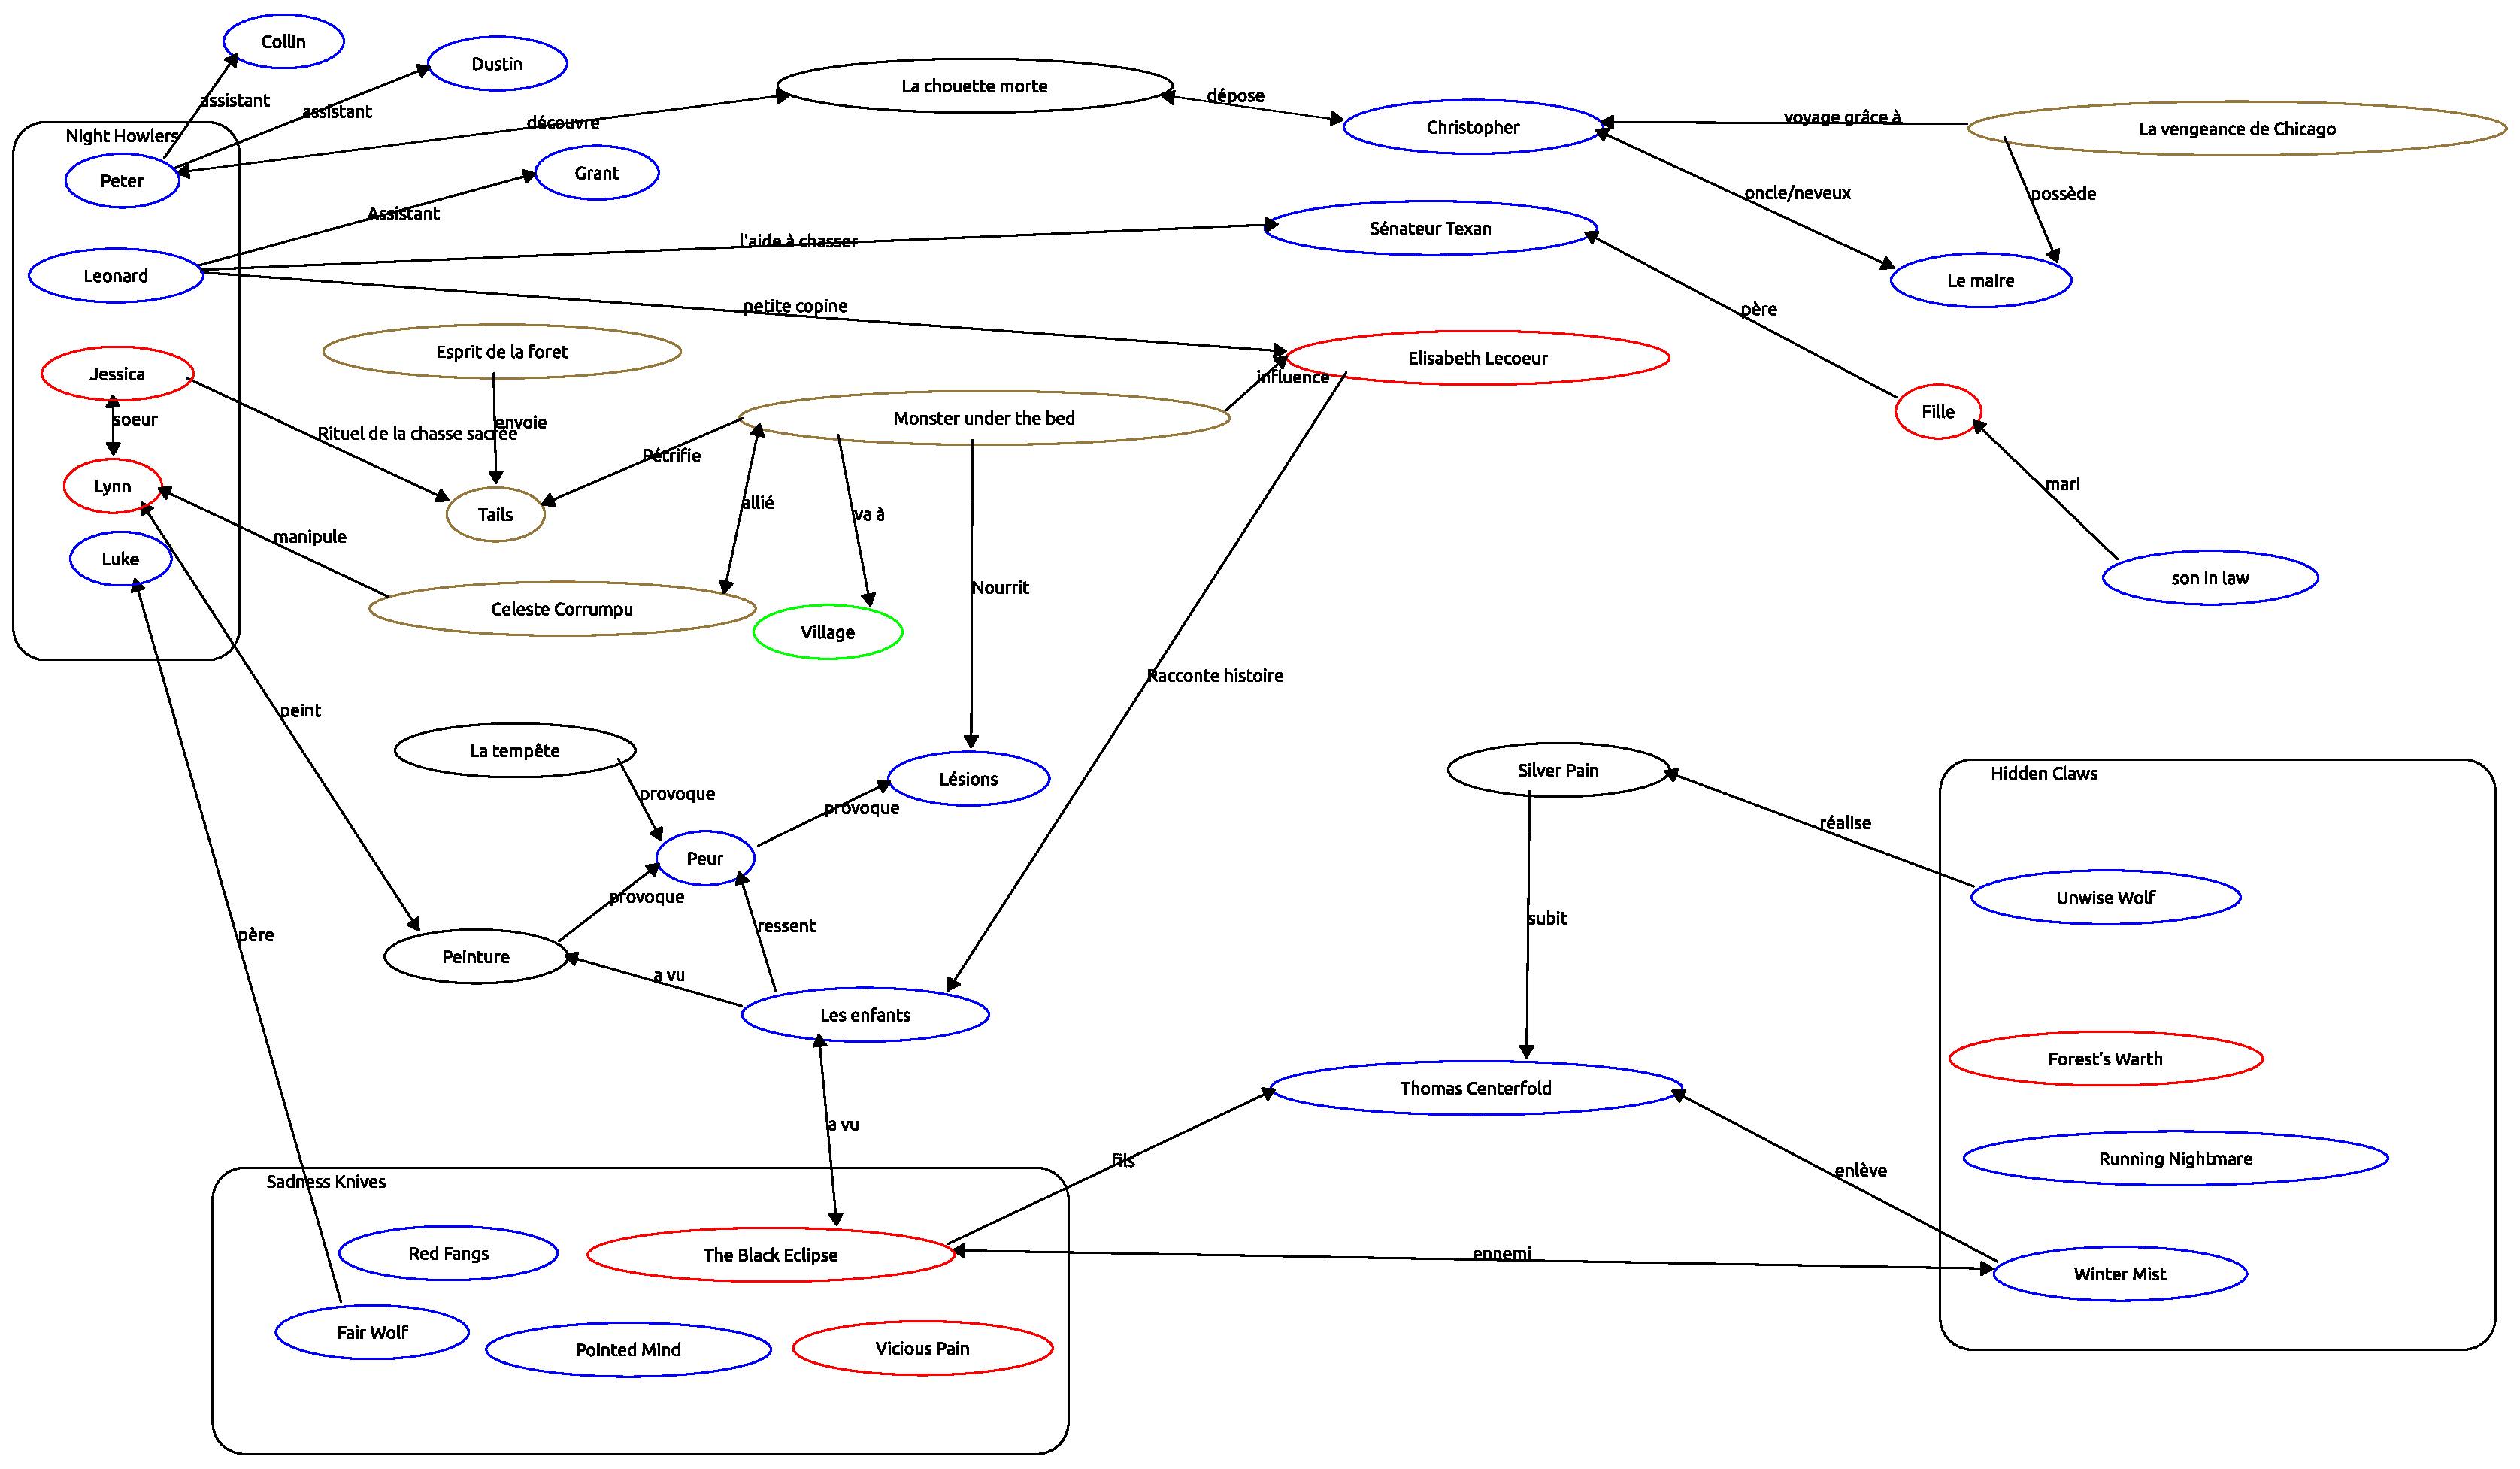
\includegraphics[width=\textwidth]{canada_2.eps}
\caption{Schéma du scénario définissant l'ensemble des relations entre les différents personnages. Image vectorielle, réaliser avec le logiciel \href{https://github.com/obiwankennedy/rmindmap}{Rmindmap}}
%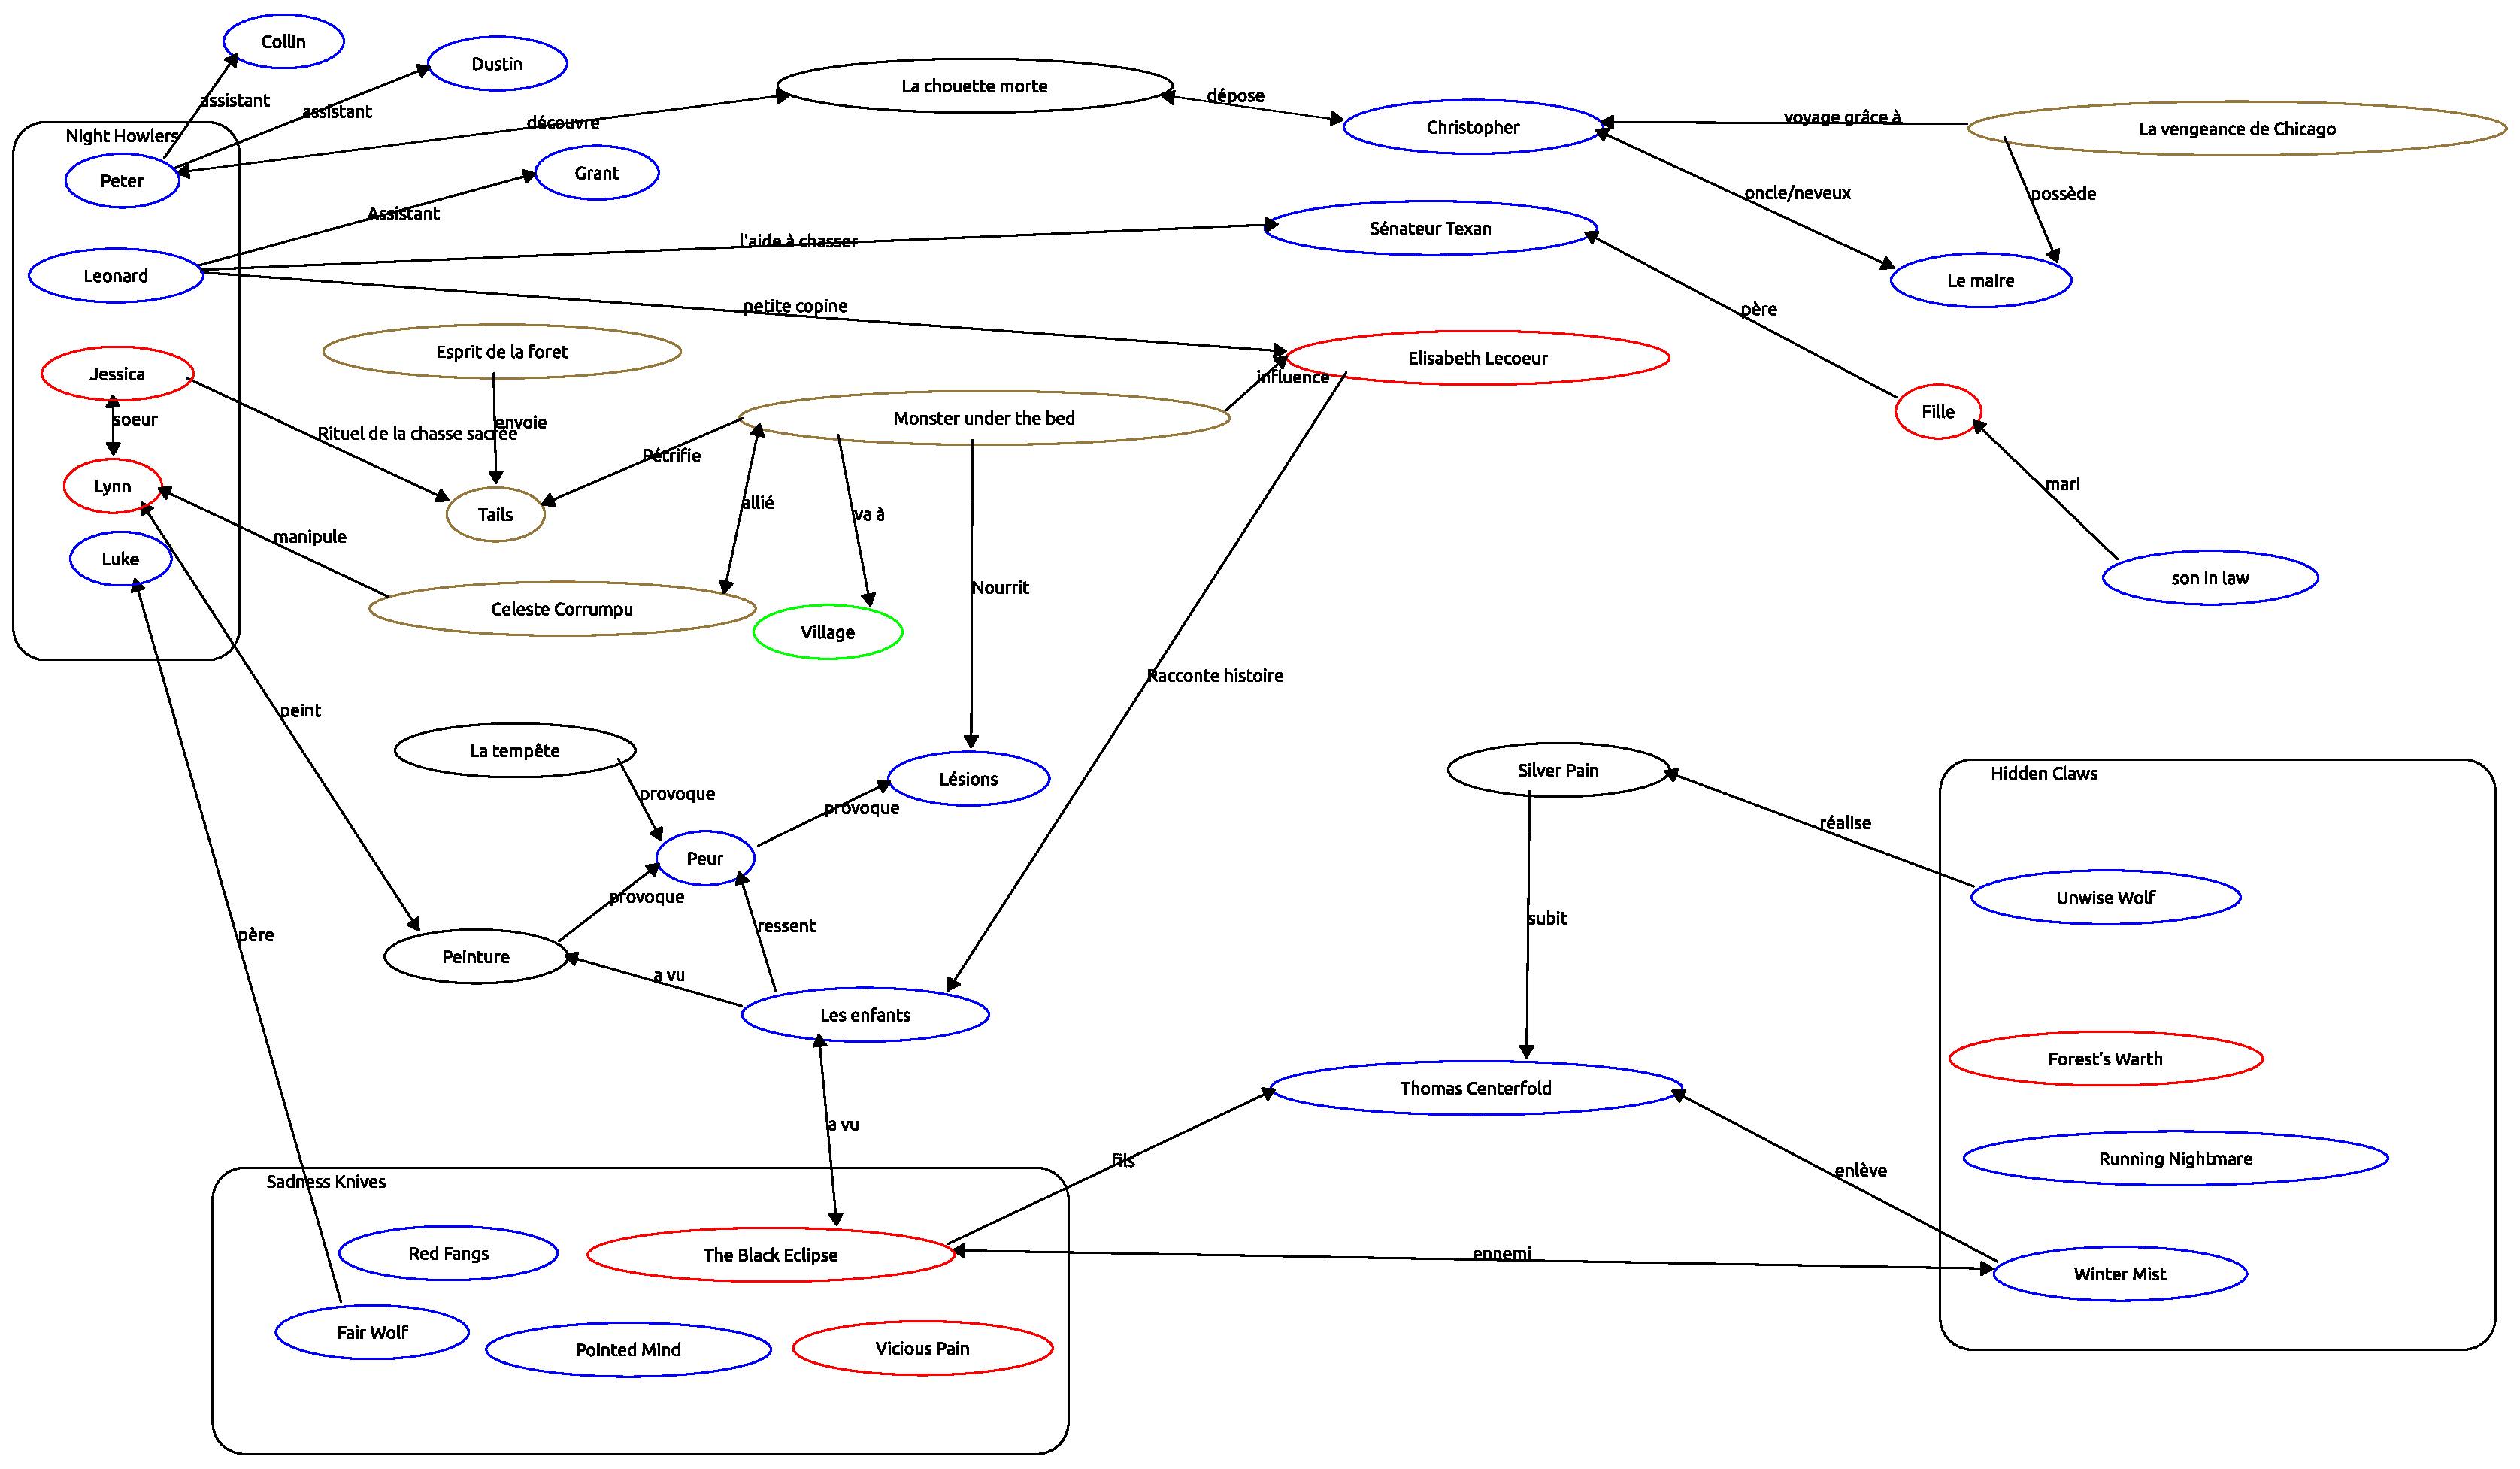
\includegraphics[width=\textwidth]{canada_2.eps}
\label{fig:mindmap}
\end{figure}

\end{flushleft}
\end{document}
